\section{Descripción General}
En este documento se desarrollarán las motivaciones, implicaciones y detalles de la implementación de este Trabajo de Fin de Grado.

El objetivo general de este proyecto ha sido el desarrollo de un videojuego educativo que sirva como apoyo para el desarrollo del Pensamiento Computacional (en adelante PC) en niños de Primaria/ESO. El PC se define como una habilidad cognitiva que permite resolver problemas utilizando estrategias computacionales\cite{tesismaria}, de las cuales se pueden extraer seis factores y sus definiciones\cite{tesismaria}:
\begin{compactitem}
    \item Abstracción: Proceso de obtener algo simple desde algo complejo, obviando los detalles.
    \item Análisis de datos: Buscar, seleccionar, organizar y analizar lógicamente los datos. 
    \item Descomposición de problemas: Descomponer problemas en otros más pequeños que pueden resolverse con mayor facilidad. 
    \item Algoritmia: Identificar instrucciones específicas y explícitas que, paso a paso, llevan acabo un proceso.
    \item Depuración de errores: Identificar y corregir los errores en la solución aportada.
    \item Generalización: Transferir un proceso de resolución de problemas a una variedad grande de problemas.
\end{compactitem}

Partiendo de esta base, se ha desarrollado el videojuego EcoRescue con el objetivo de añadir elementos jugables que ayuden a potenciar gran parte de todas estas facetas del PC. Dado que este proyecto se ha desarrollado en conjunto con otra alumna, la documentación del diseño queda fuera del alcance de este documento, sin embargo, sí que habrá referencias al Game Design Document (GDD) cuando sea preciso para ilustrar el punto que se esté desarrollando en ese momento.

EcoRescue es un videojuego que además de ser un apoyo en el desarrollo del PC, pretende ser didáctico con los temas que muestra y enseñar a los niños que lo jueguen información acerca del medio ambiente y la restauración de ecosistemas, siendo así la mecánica principal restaurar los ecosistemas en los que consisten sus niveles. Con este fin se ha contado con el apoyo de la Doctoranda en restauración de ecosistemas, \nombreproductor.

Las mecánicas de EcoRescue se pueden definir en dos fases, la de investigación y la de restauración. Al iniciar el juego, el jugador se encuentra con una lista de niveles que muestran una serie de biomas y características a restaurar, una vez entra, comenzará la fase de investigación:
\begin{compactitem}
    \item Durante la fase de investigación, el jugador puede observar un mapa cuadriculado en vista isométrica con varios biomas visibles.
    \item Encima de cada bioma, verá una burbuja con un icono (Figura \ref{fig:burbujas}) con la que deberá interactuar para aprender sobre qué le puede estar ocurriendo al bioma.
    \item Esta interacción muestra un libro con información acerca del bioma, su alteración y sus problemas (Figura \ref{fig:libro}).
    \item El jugador tendrá que completar un minijuego en el que relacione los problemas con sus posibles consecuencias (Figura \ref{fig:relations}) para demostrar que ha entendido qué es lo que le está ocurriendo al bioma.
\end{compactitem}

\begin{figure}[H]
  \centering
	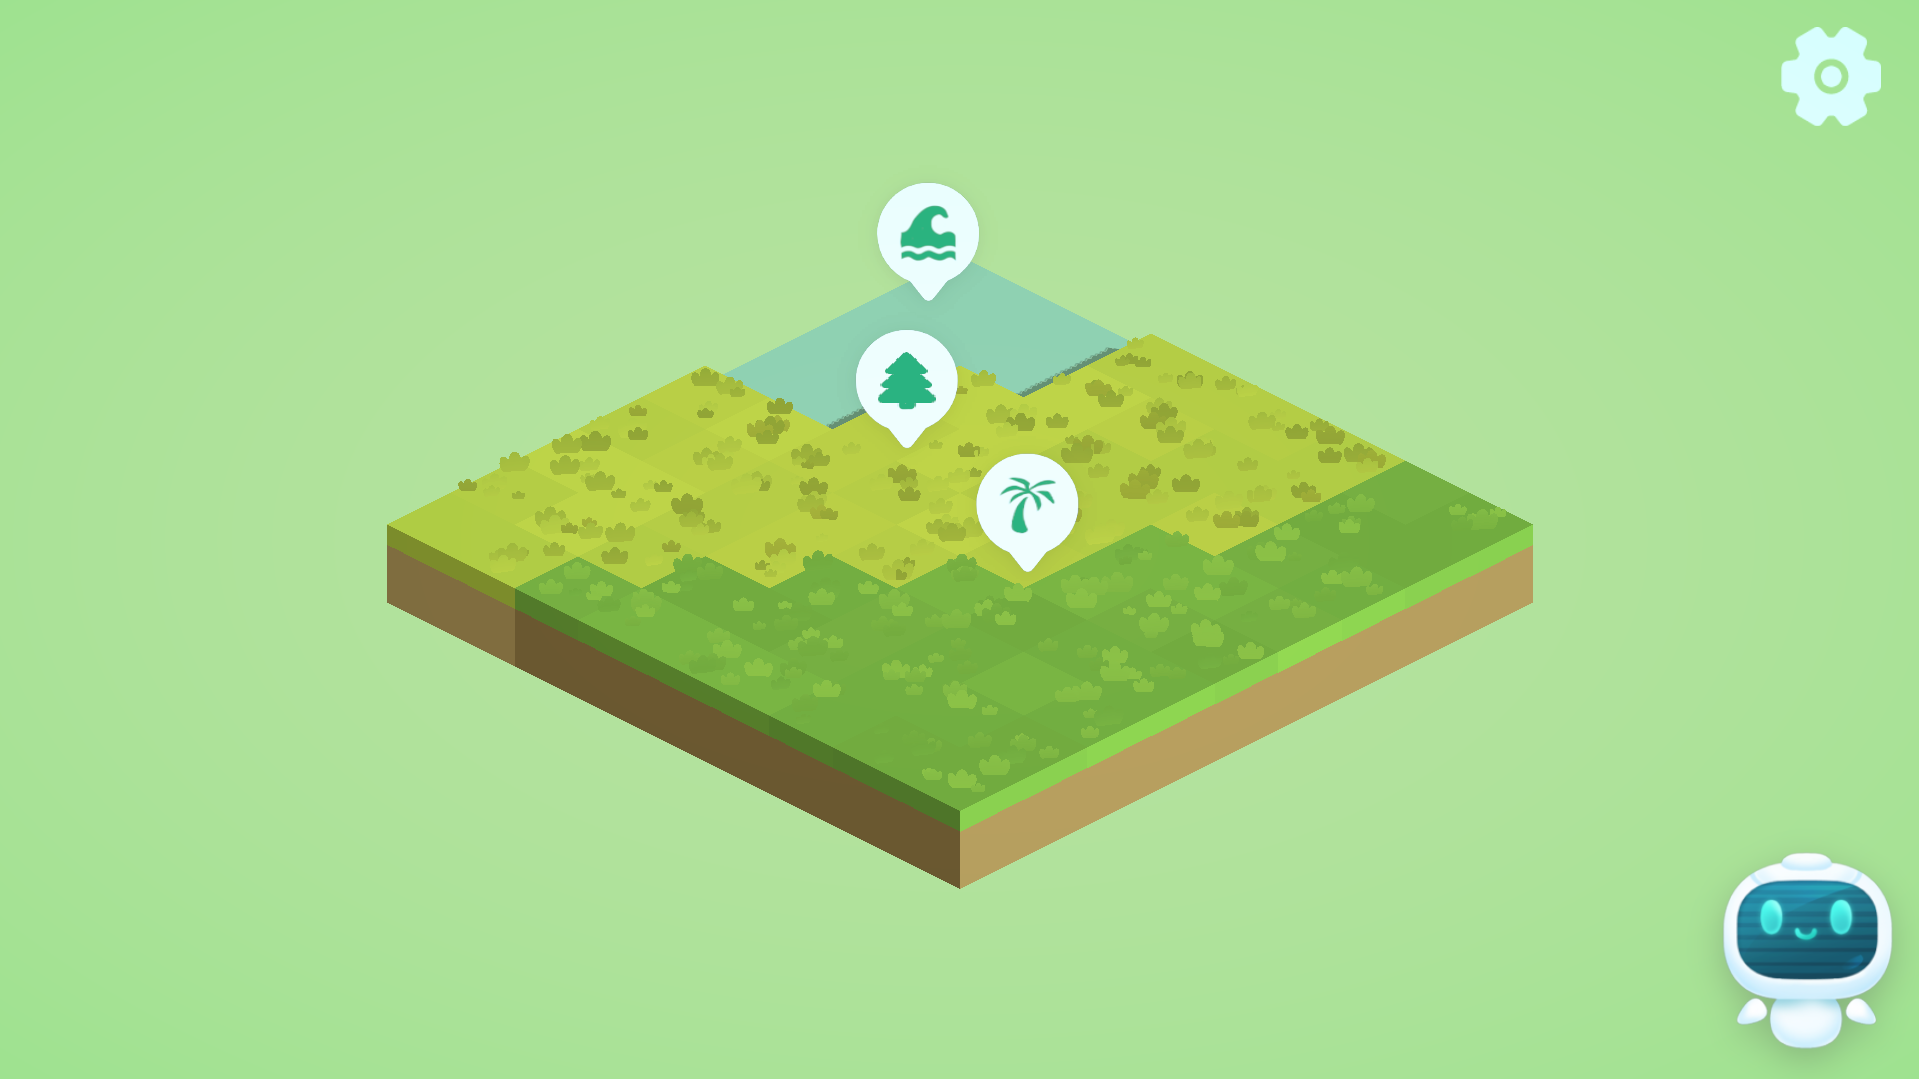
\includegraphics[width=350px,clip=true]{burbujas.png}
  \caption{Mapa con burbujas de bioma visibles}
  \label{fig:burbujas}
\end{figure}

\begin{figure}[H]
  \centering
	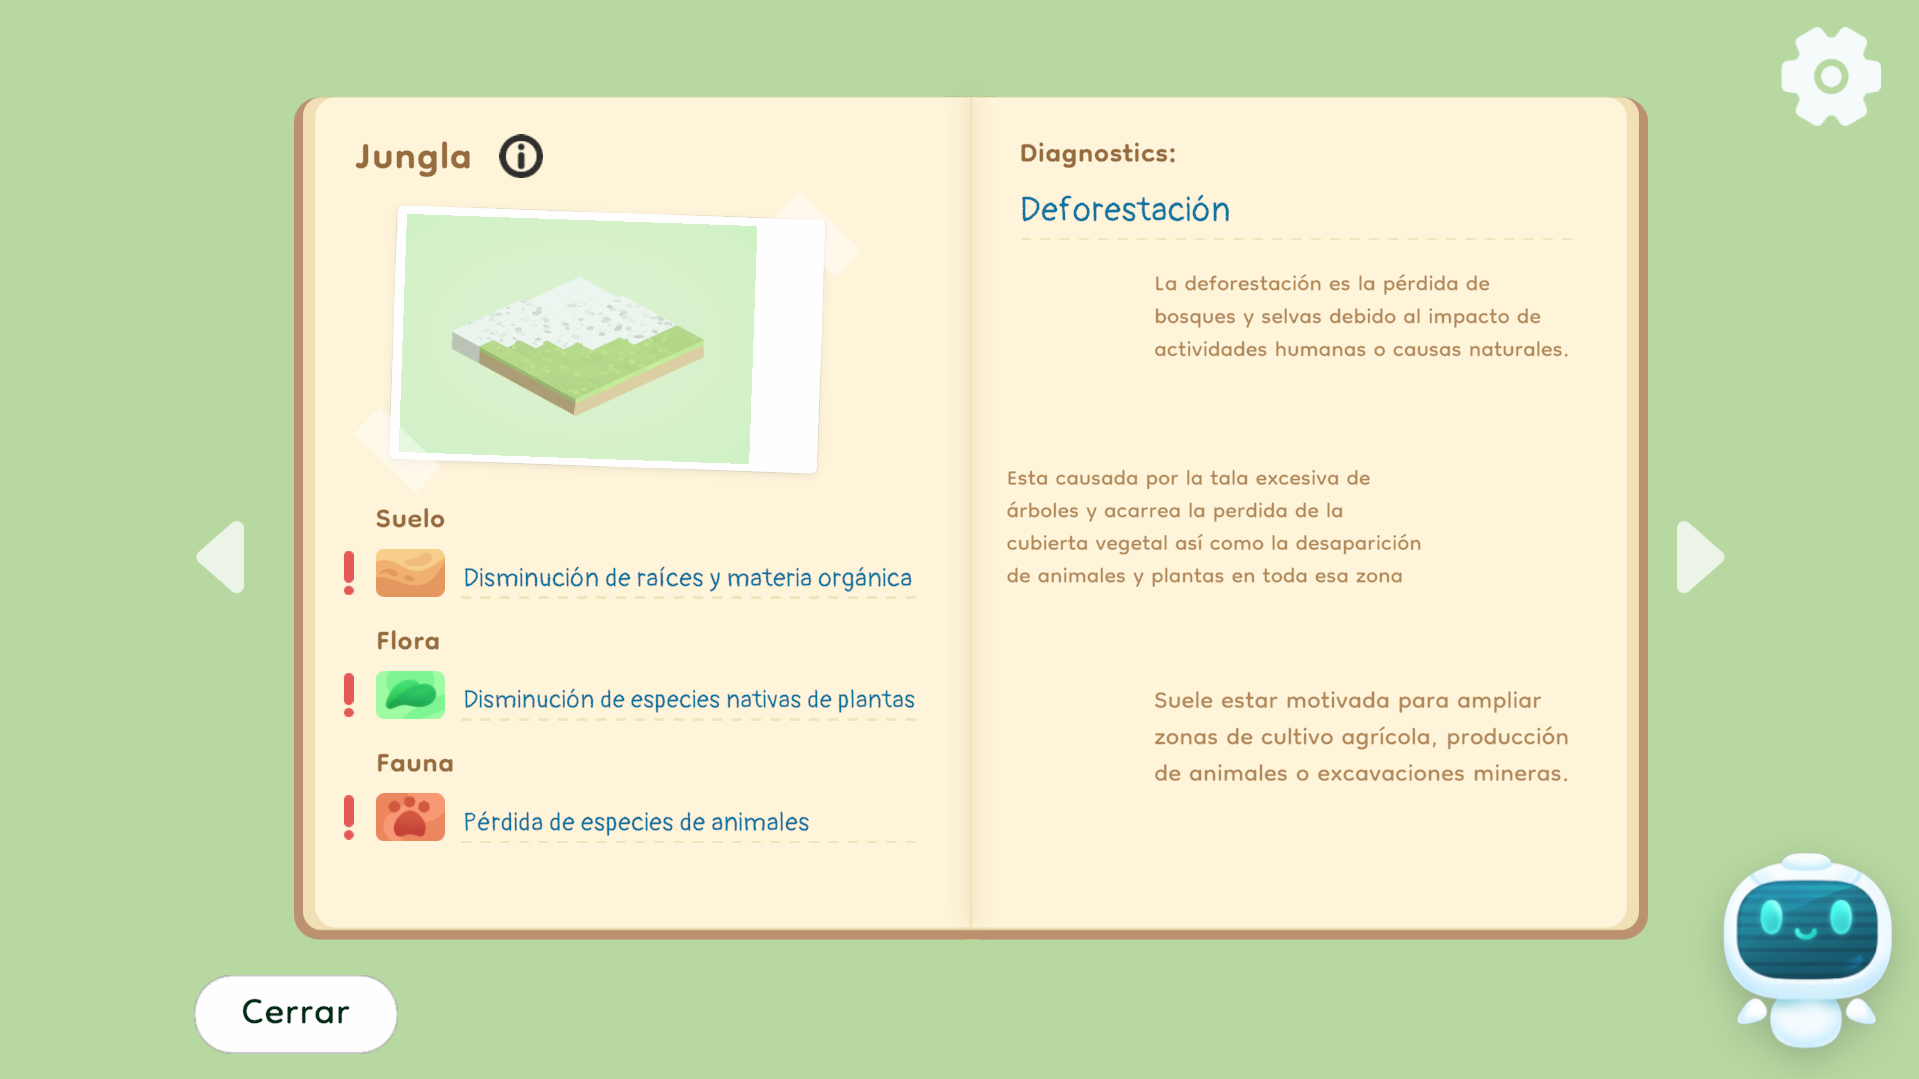
\includegraphics[width=350px,clip=true]{libro_info.png}
  \caption{Libro con información de problemas medioambientales}
  \label{fig:libro}
\end{figure}

\begin{figure}[H]
  \centering
	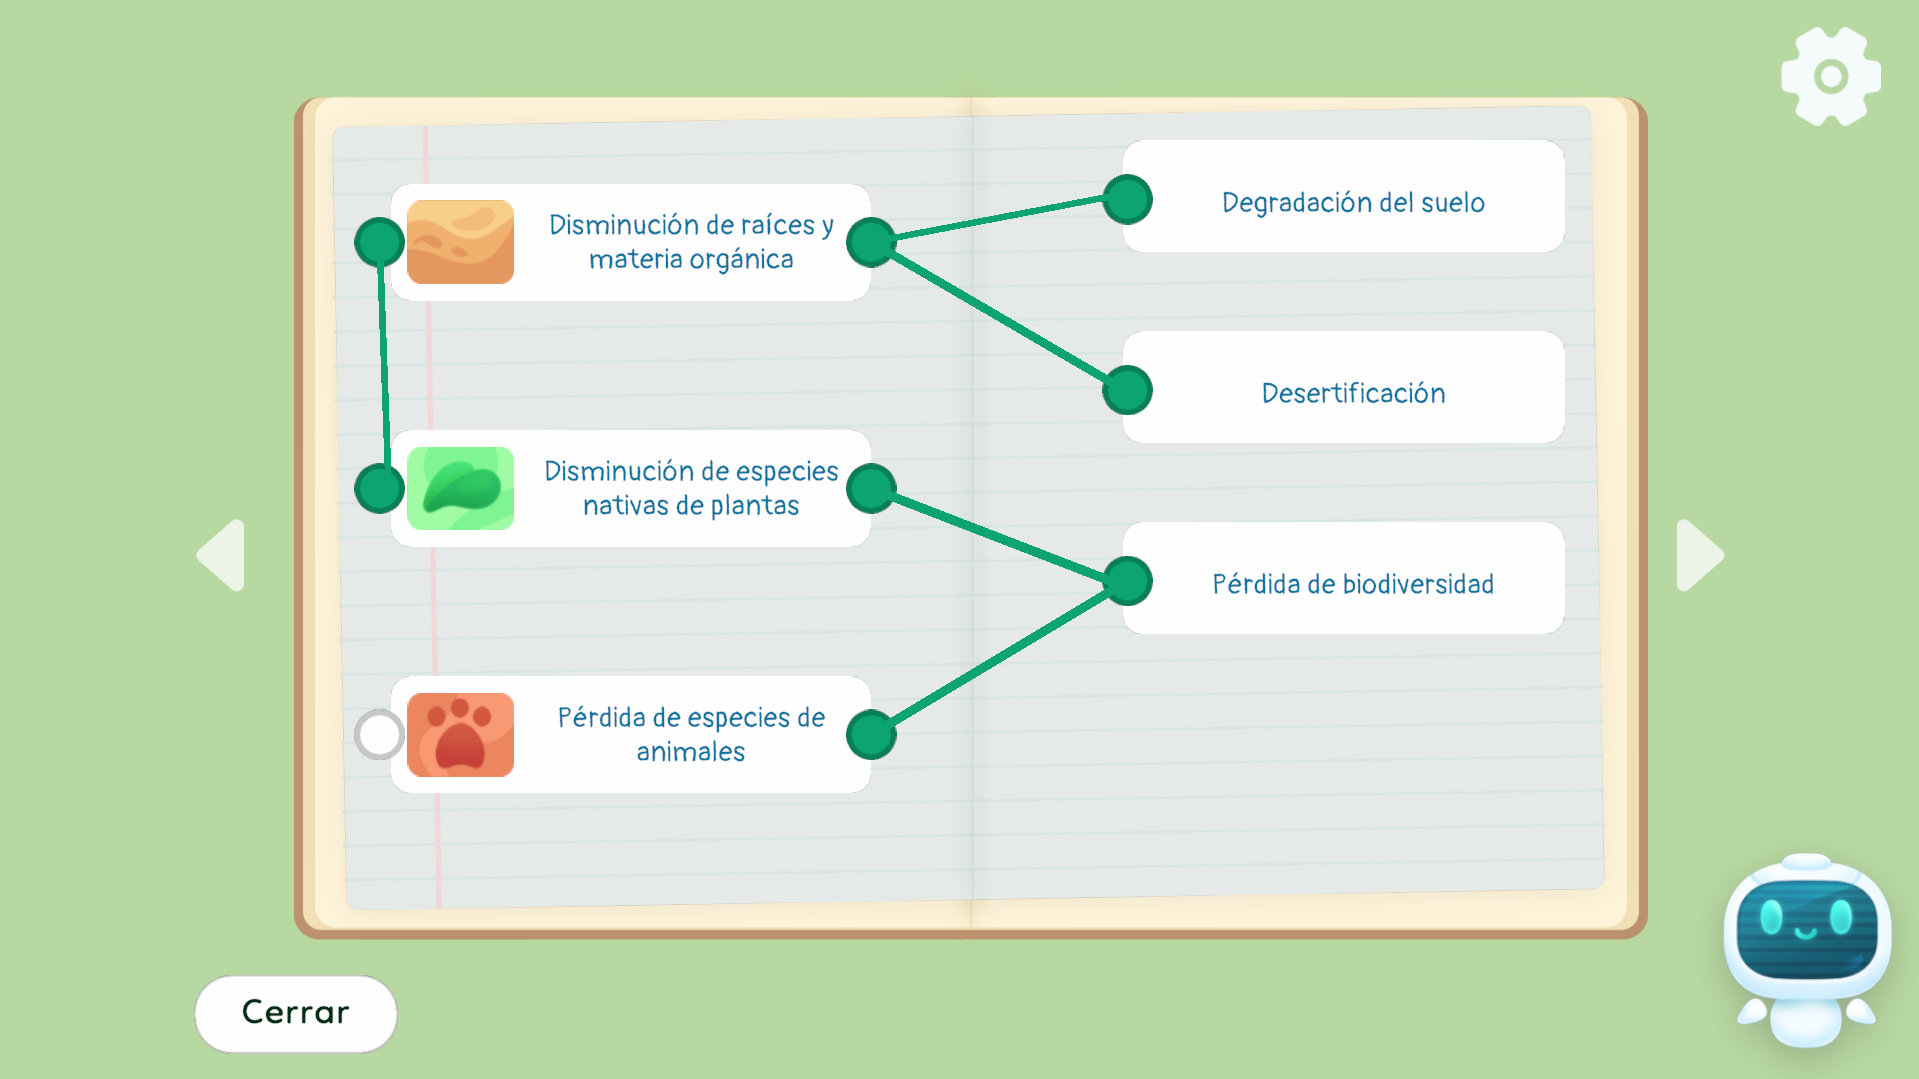
\includegraphics[width=350px,clip=true]{libro_relaciones.png}
  \caption{Libro de Relaciones Problema - Consecuencia}
  \label{fig:relations}
\end{figure}

Una vez el jugador haya demostrado que ha entendido todas las alteraciones y problemas de todos los biomas, el juego pasará a la segunda fase, la de restauración.
\begin{compactitem}
    \item Durante la fase de restauración, el jugador tendrá un presupuesto de energía para gastar en máquinas restauradoras.
    \item Cada bioma tendrá una alteración, que a su vez estará compuesta de 2-3 fases, cada una definida por un problema distinto (Deforestación, Desertificación, Sobrepesca…)
    \item El jugador deberá comprar máquinas restauradoras de la tienda y colocarlas en el bioma para que puedan hacer efecto, los distintos efectos de estas restaurarán el ecosistema de una forma u otra.
    \item La jugabilidad radica en que el jugador tendrá distintas opciones de máquinas (tres) por cada fase de cada bioma, y cada opción tendrá un efecto distinto, teniendo en cuenta la información que ha adquirido durante la primera fase, y la información que proporciona la tienda acerca del efecto de la máquina, el jugador deberá hacer una elección que le permita restaurar el ecosistema por un coste apropiado, con el objetivo de no quedarse sin presupuesto antes de terminar todas las fases de todos los biomas.
\end{compactitem}

Teniendo en cuenta las estrategias del PC y las mecánicas del juego, podemos asimismo definir una tabla (Tabla \ref{fig:tablaPCMecanicas}) que las relacione entre sí, dejando claro de qué forma se pretende ayudar a potenciar el PC en los jugadores.
\raggedbottom
\begin{table}[H]
\begin{center}
\setlength{\tabcolsep}{5pt}
\renewcommand{\arraystretch}{1.2}
\begin{tabular}{ | m{8em} | m{30em} | } 
  \hline
  Estrategia & Mecánica \\ 
  \hline
  Abstracción & A la hora de realizar los diagramas de correlación entre indicadores (datos) y sus consecuencias, se reduce al mínimo imprescindible la explicación del contexto de la alteración del ecosistema. \\ 
  \hline
  Análisis de Datos & La fase de investigación muestra una serie de datos que posteriormente el jugador analiza para poder correlacionarlos con consecuencias. \\ 
  \hline
  Descomposición de problemas & Un nivel está visiblemente desglosado en diferentes tareas y subtareas. Para completar el nivel es necesario restaurar todos los biomas y para restaurar cada bioma hay que finalizar todas las fases del plan de restauración (que pueden considerarse tareas a cumplimentar). \\ 
  \hline
  Algoritmia & A la hora de restaurar un ecosistema, está todo claramente separado de forma secuencial. Incluso el propio nivel se desarrolla de forma secuencial. \\ 
  \hline
  Depuración de Errores & Es posible cometer errores y es importante detectarlos y subsanarlos a tiempo. La idea es dejar cierto margen para que los jugadores puedan echarse atrás y arreglar los fallos. \\ 
  \hline
    & El jugador tiene recursos (moneda) limitados y debe hacer un buen uso de ellos para poder completar los niveles, si se queda sin dinero, deberá volver a intentarlo para poder minimizar el gasto. \\ 
  \hline
  Generalización & A menudo las alteraciones de los ecosistemas tienen factores en común, a lo largo del progreso en el videojuego los jugadores podrán ir discerniendo que existen muchas correlaciones entre alteraciones y sus consecuencias. Por ejemplo: Si hay un problema con el suelo (del tipo que sea) la flora no va a poder prosperar correctamente y si la flora no está en sus condiciones óptimas, la fauna tampoco lo estará. \\ 
  \hline
\end{tabular}
\centering
\caption{Relaciones entre Estrategias del PC con mecánicas del videojuego.}
\label{fig:tablaPCMecanicas}
\end{center}
\end{table}


\section{Motivación}

La motivación para el desarrollo de EcoRescue surge de proponerle a \nombretutor el desarrollo de un videojuego junto con otra alumna, \nombrecoautor. \nombretutor aceptó la propuesta y planteó que el videojuego formase parte de una iniciativa Europea para desarrollar videojuegos que ayuden a fomentar el PC en niños y adolescentes.

Esta iniciativa nace a a raíz del Plan de Acción de Educación Digital 2021-2027 de la Comisión Europea\cite{europaPlan}, además de verse reforzada en España por los Reales Decretos 157/2022\cite{boePrimaria} y 217/2022\cite{boeSecundaria}, del 1 y 19 de marzo del 2022 respectivamente, que abogan por la inclusión del desarrollo del PC como competencia obligatoria a enseñar en las etapas de Educación Primaria y Secundaria Obligatoria.

Como se ha mencionado anteriormente, además de servir para desarrollar el PC, uno de los objetivos del proyecto es informar sobre la importancia de cuidar el medioambiente y de como distintos indicadores y alteraciones pueden afectar negativamente a estos. De esta forma, el juego puede ayudar a niños y adolescentes a relacionar consecuencias del sistema productivo de la sociedad actual con los daños que sufren actualmente nuestros ecosistemas y entornos naturales. A su vez, ilustra de forma eficiente como interaccionan diferentes ecosistemas entre sí y como se relacionan sus diferentes elementos: fauna, flora y el soporte natural. Además, el juego aporta una versión optimista de como entornos que se consideran destruidos se pueden recuperar mediante la intervención y tecnología adecuados. 

Este enfoque es relevante dado que según los Reales Decretos mencionados anteriormente\cite{boePrimaria}\cite{boeSecundaria} se estipula que en lo relacionado al Conocimiento del Medio, Biología y Geología se buscará fomentar el razonamiento y pensamiento crítico (computacional) para resolver problemas o dar explicación a procesos de la vida cotidiana relacionados.

Finalmente habría que considerar también la motivación adicional de aprender el uso de nuevas tecnologías mediante el desarrollo de un proyecto, que tendría como objetivo el propio aprendizaje y la acumulación de experiencia de llevar un proyecto desde su etapa de concepción hasta validarlo con un grupo de alumnos de instituto.